\documentclass{../grid-link-report}
\usepackage{graphicx} % for \resizebox
\usepackage{float}

\SetClassAssetsDir{../class-assets}
\newcommand{\projectassetsdir}{../project-assets}
\newcommand{\analysisdir}{report-assets/analysis}

\project{Clements Gap BESS}
\client{Enzen}
\title{Dynamic Model Acceptance Report (PSSE) - Charging}
\docnumber{CGBESS-GR-RPT-009}
\issueddate{16 May 2025}
\revision{1-0-0}
\revisionhistorycsvpath{report-assets/revisionhistory.csv}
\clientlogopath{\projectassetsdir/client-logo.png}

\colorlet{Line}{red}
\colorlet{Intermediate}{yellow}
\colorlet{Low}{green}


\begin{document}
	% Draft commands
%	\adddraftstamp
%	\listoftodos
	
	\frontmatter
	\maketitle
	
	\makedisclaimer
	\clearpage
	\tableofcontents
	\makerevisionhistorypage
	%\makeaboutgridlink
	
	\mainmatter
	
	
	\chapter{Purpose}
	This report has been prepared to assess the accuracy, consistency and robustness of the \ac{RMS} model prepared in PSSE to represent \ac{CGBESS} between upper and lower boundaries of system strength. The results obtained as part of this assessment also provide a basis for comparison between the proposed PSSE (being an \ac{RMS} platform) and PSCAD (being and \ac{EMT} platform) models. This assessment was conducted in accordance with the requirements of the \ac{DMAT} Guidelines published by the Australian Energy Market Operator (AEMO) in June 2024 \cite{dmat-spec}.
	
	The results of this assessment provide confidence that the PSSE model prepared to represent \ac{CGBESS} is usable and numerically robust under all operating conditions that can be reasonably expected.
	
	
	\chapter{Project Overview}
	The Heywood Battery Energy Storage System (HEYWOODBESS) is a $\pm~285MW/1140MWh$ Battery Energy Storage Project, is located 5 km from the town of Heywood and 300 km west of Melbourne in Victoria as shown in Figure~\ref{fig:project-location}. The project is expected to connect directly to the existing 275 kV Heywood terminal station via a single high voltage cable.

HEYWOODBESS will include 92 SMA Sunny Central 4.6 MVA (SCS 4600 UP-S) converters which will be connected to two 275/33/33kV, 160MVA three winding transformers through a 33kV reticulation system. Each converter will have a dedicated 33/0.69kV, 4.6 MVA step up transformer.


\begin{figure}[H]
	\centering
	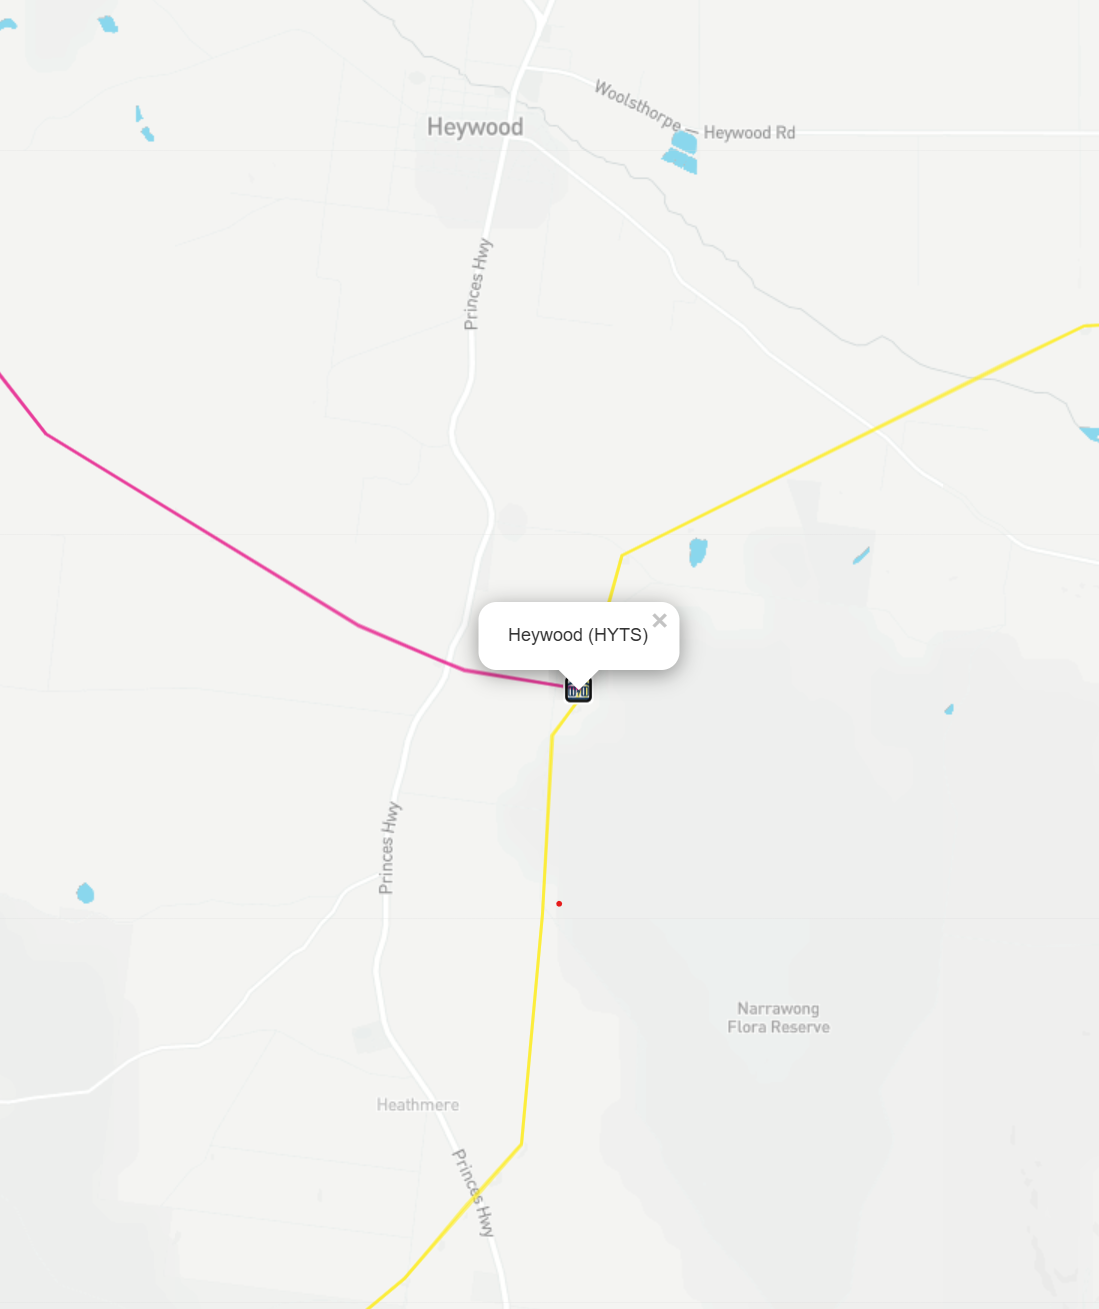
\includegraphics[width=0.7\textwidth]{\projectassetsdir/project-location.png} % Change example-image-a to the filename of your image
	\caption{Project location}
	\label{fig:project-location}
\end{figure}


	
	\chapter{Results}
	
	All simulations have been performed on version v1-0-0 of the \ac{CGBESS} PSSE model.
	
	The following site-specific values have been used in performing the \ac{DMAT} tests:
	
	\begin{itemize}
		\item Maximum fault level and associated \ac{SCR}: 1068 MVA and 17.8.
		\item Minimum fault level and associated \ac{SCR}: 510 MVA and 8.5.
	\end{itemize}
	
	Figure \ref{fig:PSSEmodelSLD}. shows the PSS/E model single line diagram including layout of the generating system and the infinite bus grid model.
	
	\begin{figure}[H]
		\centering
		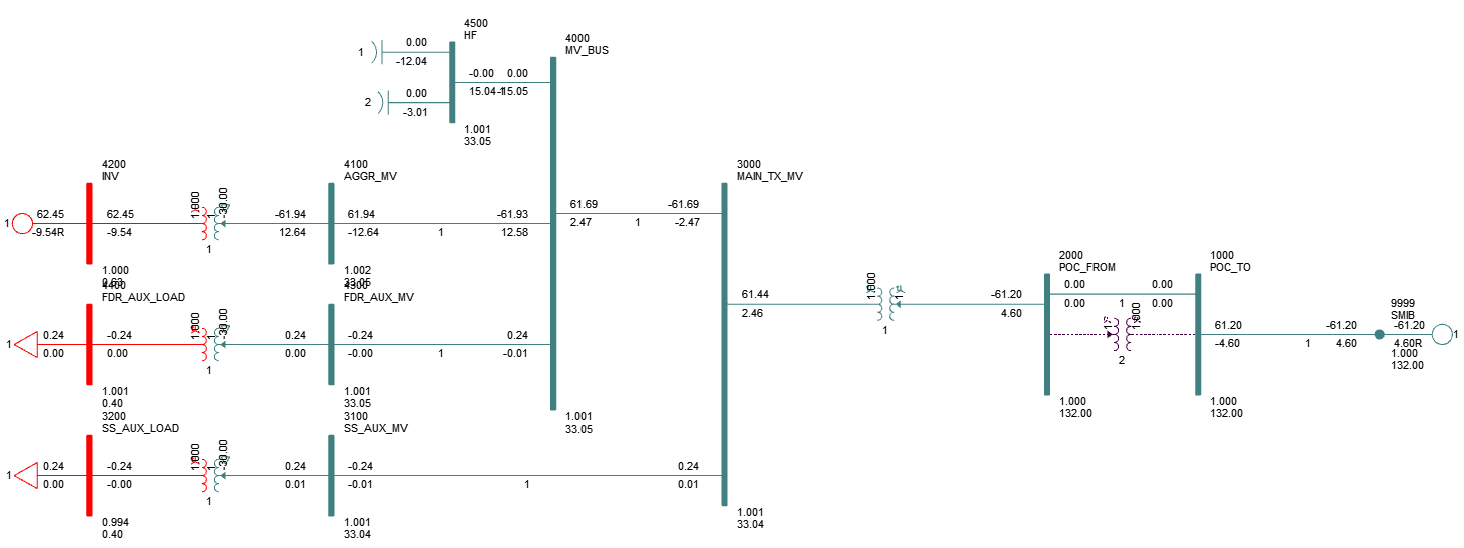
\includegraphics[width=0.7\linewidth]{\projectassetsdir/PSSEsld.png}
		\caption{PSSE model single line diagram}
		\label{fig:PSSEmodelSLD}
	\end{figure}
	
	Further detail regarding the detailed parameters of plant equipment has been outlined in the Clements Gap BESS Releasable User Guide (RUG).

	\subsection{Note On PLL Instability}
	\label{foreword on instability}
	
	For a select number of balanced faults, TOV, grid voltage disturbance tests and a single phase angle step test, the response seen in PSS/E is understood to be a result of potential PLL instability seen on fault clearance. Furthermore, we believe the reason this appears in PSS/E is related to differences in RMS and EMT modelling platforms - as Spike Mitigation algorithms implemented in PSS/E meant to filter out discontinuities appear to influence this response. Please refer to the supporting technical note "Clements Gap BESS - Spike mitigation and PLL issue at low SCR" \cite{tech-note}.
	
	
	\section{Balanced faults - DMAT 3.2.4}
	\label{sec:balanced-faults}
	Balanced faults are applied to the Connection Point as shown in Figure~\ref{fig:balanced-fault-diagram}. The fault impedance, $Z_{\text{fault}}$, is selected using one of two strategies, as required by the given test:

\begin{itemize}
	\item As a ratio of the fault impedance to the grid impedance. This could be used to specify an intended depth of fault (before generator response).
	\item Using exact values for $R_{\text{fault}}$ and $X_{\text{fault}}$.
\end{itemize}

\begin{figure}[h]
	\centering
	\newcommand{\bushere}[3]{% length, text above, text below}
% Optional arguments do nto work in paths
%
% starting point; draw an edge and then two nodes
% save the position
coordinate(tmp)
% go up and do an edge down
++(0,#1) node[anchor=base, font=\footnotesize]{#2} edge[ultra thick] ++(0, {-2*#1})
% edges do not move the current point, go down to position the node
++(0,{-2*#1}) node[below]{#3}
% go back to where we started
(tmp)
}

\ctikzset{sources/fill=gray!20, resistors/fill=gray!20}
\resizebox{0.65\linewidth}{!}{ % Set width to \linewidth
	\begin{tikzpicture}[semithick]% default line width
		% Buses and branches
		\draw (0,0)
		node[left, font=\footnotesize]{Generator} ++(1.5,0) \bushere{1.5}{Connection Point}{} coordinate(poc);
		\draw (poc)
		-- ++ (1,0) to[generic, l={$Z_{\text{grid}}$}, resistors/width=2] ++ (4,0)
		-- ++ (1,0)
		\bushere{1.5}{Infinite Bus}{} coordinate(infinite bus);
		% One load (start from the coord load, go up)
		\ctikzset{bipoles/border margin=0.5}% See manual section 3.1.2
		\draw (infinite bus) -- ++(1,0) node[vsourcesinshape, rotate=90]{} ++(0.5,0) node[right]{$V_{\text{grid}}$};
		\draw (poc) -- ++(-1,0) node[vsourcesinshape, rotate=90]{};
		% Fault
		\draw[red, font=\footnotesize] (poc) ++(0, -0.7) -- ++(0.7,0) -- ++(0,-1) node[ground]{} ++(0.6,0.2) node[]{$Z_{\text{fault}}$};
		
	\end{tikzpicture}
}






	\caption{Fault application methodology}
	\label{fig:balanced-fault-diagram}
\end{figure}
	
	The full list of balanced faults assessed can be found in Table \ref{tab:balanced-faults-test-suite}.
	
	{
		\fontsize{5}{7}\selectfont
		\autoscaledlongtable
		{Balanced faults test suite}
		{tab:balanced-faults-test-suite}
		{\projectassetsdir/test-suite-tables/PSSE-DMAT-CRG/324-325-Faults-CRG-balanced-test-table.csv}
	}
	
	Results for DMAT 3.2.4 can be found in Appendix \nameref{Appendix A: Balanced faults}.
	
	Please refer to section \ref{foreword on instability} for discussion on the response of tests p5,p6,p17 and p29.
	
	All other tests conducted produced results that were found to be acceptable.
	

	\section{Multiple fault ride-through (PSSE) - DMAT 3.2.7}
	
	Multiple Fault Ride Through (MFRT) tests are performed in the same manner as balanced and unbalanced faults. However, instead of a single fault being applied, a selection of faults with different characteristics (balanced/unbalanced, different fault impedances, different durations) are selected to demonstrate the ability to withstand many disturbances.

As with balanced and unbalanced faults, the faults are all applied to the Connection Point as shown in Figure~\ref{fig:mfrt-diagram}.

\begin{figure}[h]
	\centering
	\newcommand{\bushere}[3]{% length, text above, text below}
% Optional arguments do nto work in paths
%
% starting point; draw an edge and then two nodes
% save the position
coordinate(tmp)
% go up and do an edge down
++(0,#1) node[anchor=base, font=\footnotesize]{#2} edge[ultra thick] ++(0, {-2*#1})
% edges do not move the current point, go down to position the node
++(0,{-2*#1}) node[below]{#3}
% go back to where we started
(tmp)
}

\ctikzset{sources/fill=gray!20, resistors/fill=gray!20}
\resizebox{0.65\linewidth}{!}{ % Set width to \linewidth
	\begin{tikzpicture}[semithick]% default line width
		% Buses and branches
		\draw (0,0)
		node[left, font=\footnotesize]{Generator} ++(1.5,0) \bushere{1.5}{Connection Point}{} coordinate(poc);
		\draw (poc)
		-- ++ (1,0) to[generic, l={$Z_{\text{grid}}$}, resistors/width=2] ++ (4,0)
		-- ++ (1,0)
		\bushere{1.5}{Infinite Bus}{} coordinate(infinite bus);
		% One load (start from the coord load, go up)
		\ctikzset{bipoles/border margin=0.5}% See manual section 3.1.2
		\draw (infinite bus) -- ++(1,0) node[vsourcesinshape, rotate=90]{} ++(0.5,0) node[right]{$V_{\text{grid}}$};
		\draw (poc) -- ++(-1,0) node[vsourcesinshape, rotate=90]{};
		% Fault
		\draw[red, font=\footnotesize] (poc) ++(0, -0.7) -- ++(0.7,0) -- ++(0,-1) node[ground]{} ++(0.6,0.2) node[]{$Z_{\text{fault}}$};
		
	\end{tikzpicture}
}






	\caption{MFRT application methodology}
	\label{fig:mfrt-diagram}
\end{figure}
	
	The full list of multiple fault ride through PSSE tests assessed can be found in Table \ref{tab:mfrt-psse-test-suite}.
	
	{
		\renewcommand{\arraystretch}{1.2}
		\setlength{\tabcolsep}{5pt}
		
		\begin{longtable}{|C{1cm}|C{4cm}|C{4cm}|C{4cm}|C{4cm}|}
			\caption{MFRT test suite} \label{tab:mfrt-psse-test-suitee} \\
			\hline
			\textbf{Test} & \textbf{Fault Types} & \textbf{Fault Durations} & \textbf{Time Between Faults} & \textbf{Fault Impedance $Z_f/Z_s$}\\
			\hline
			S1 & 3PHG, 3PHG, 3PHG, 3PHG, 3PHG, 3PHG, 3PHG, 3PHG, 3PHG, 3PHG, 3PHG, 3PHG, 3PHG, 3PHG, 3PHG & 0.43, 0.12, 0.12, 0.12, 0.12, 0.22, 0.12, 0.22, 0.12, 0.22, 0.22, 0.22, 0.22, 0.12, 0.12 & 5, 0.5, 0.01, 1.5, 0.2, 7, 1, 0.2, 0.75, 2, 0.5, 0.01, 10, 2 & 2, 1, 2, 0, 3.5, 1, 3.5, 0.2, 1, 1, 0.2, 2, 0, 0.2, 1  \\
			\hline
			S2 & 3PHG, 3PHG, 3PHG, 3PHG, 3PHG, 3PHG, 3PHG, 3PHG, 3PHG, 3PHG, 3PHG, 3PHG, 3PHG, 3PHG, 3PHG & 0.22, 0.22, 0.12, 0.12, 0.22, 0.12, 0.43, 0.22, 0.12, 0.22, 0.12, 0.22, 0.12, 0.12, 0.12 & 0.2, 10, 2, 0.2, 0.75, 0.5, 1, 0.5, 2, 0.01, 7, 5, 1.5, 3 & 1, 2, 2, 0.2, 1, 1, 2, 0, 0.2, 1, 1, 0.2, 3.5, 0, 3.5  \\
			
			\hline
			S3 & 3PHG, 3PHG, 3PHG, 3PHG, 3PHG, 3PHG, 3PHG, 3PHG, 3PHG, 3PHG, 3PHG, 3PHG, 3PHG, 3PHG, 3PHG & 0.12, 0.22, 0.22, 0.12, 0.43, 0.22, 0.12, 0.22, 0.12, 0.12, 0.12, 0.12, 0.12, 0.22, 0.22 & 0.2, 5, 1.5, 2, 3, 1, 0.5, 0.5, 0.75, 10, 7, 0.2, 0.01, 0.01 & 1, 0.2, 2, 0, 3.5, 1, 0, 1, 1, 0.2, 0.2, 3.5, 1, 2, 2  \\
			
			\hline
			S4 & 3PHG, 3PHG, 3PHG, 3PHG, 3PHG, 3PHG, 3PHG, 3PHG, 3PHG, 3PHG, 3PHG, 3PHG, 3PHG, 3PHG, 3PHG & 0.12, 0.22, 0.12, 0.22, 0.12, 0.43, 0.12, 0.12, 0.22, 0.22, 0.22, 0.12, 0.12, 0.22, 0.12 & 3, 5, 0.2, 2, 10, 1.5, 0.75, 0.01, 0.5, 0.01, 1, 2, 0.2, 0.5 & 1, 2, 0.2, 2, 2, 1, 1, 3.5, 1, 0.2, 1, 3.5, 0, 0, 0.2  \\
			
			\hline
			S5 & 3PHG, 3PHG, 3PHG, 3PHG, 3PHG, 3PHG, 3PHG, 3PHG, 3PHG, 3PHG, 3PHG, 3PHG, 3PHG, 3PHG, 3PHG & 0.12, 0.12, 0.43, 0.22, 0.22, 0.12, 0.12, 0.12, 0.22, 0.12, 0.22, 0.12, 0.22, 0.22, 0.12 & 0.2, 7, 1, 0.5, 3, 0.5, 2, 0.75, 0.01, 1.5, 0.01, 5, 0.2, 2 & 1, 0, 3.5, 0.2, 2, 0.2, 1, 3.5, 1, 2, 2, 1, 0, 0.2, 1 \\
			
			\hline
	\end{longtable}}
	
	Results for DMAT 3.2.6 can be found in \nameref{Appendix B: Multiple fault ride-through tests}.
	
	It was observed for test for MFRT test S5 that the generating system trips as a result of frequency protection. This was found to be a numerical issue with PSS/E whereby an extreme frequency disturbance is observed on fault inception (at approximately t=35s) for an extended period of time and the inverter protection then responds as expected. All other tests conducted produced acceptable results.

	All other tests conducted produced results that were acceptable.
	

	\section{Temporary over-voltage - DMAT 3.2.9}
	

	Temporary Over-Voltage tests assess the ability of the generator to ride through high voltage disturbances and supply the correct amount of inductive reactive current. To perform these tests, the appropriate $V_{\mathrm{grid}_{\mathrm{initial}}}$
is first identified to achieve $V_{\mathrm{POC}_{\mathrm{initial}}}$ given the required initial $P_{\mathrm{POC}}$, $Q_{\mathrm{POC}}$, SCR and X/R conditions. 

A shunt capacitor is then inserted at the Connection Point, sized such that $V_{\mathrm{POC}_{\mathrm{TOV}}} = k_{\mathrm{OV}} * V_{\mathrm{POC}_{\mathrm{initial}}}$, where $k_{\mathrm{OV}}$ is the desired percentage increase in $V_{\mathrm{POC}}$.

The test is then performed by initialising the system with the shunt capacitor out of service, then switching it in for the intended disturbance duration, as shown in Figure~\ref{fig:smib-tov-diagram}.

It should be noted that due to the dynamics of capacitor switching, the initial instantaneous voltage spike may appear filtered and not reach $k_{\mathrm{OV}} * V_{\mathrm{POC}_{\mathrm{initial}}}$. The settled $P_{\mathrm{POC}}$ will typically also be lower than this value due to the inductive reactive current support of the generator.

\begin{figure}[h]
	\centering
	\newcommand{\bushere}[3]{% length, text above, text below}
% Optional arguments do nto work in paths
%
% starting point; draw an edge and then two nodes
% save the position
coordinate(tmp)
% go up and do an edge down
++(0,#1) node[anchor=base, font=\footnotesize]{#2} edge[ultra thick] ++(0, {-2*#1})
% edges do not move the current point, go down to position the node
++(0,{-2*#1}) node[below]{#3}
% go back to where we started
(tmp)
}

\ctikzset{sources/fill=gray!20, resistors/fill=gray!20}
\resizebox{0.65\linewidth}{!}{ % Set width to \linewidth
	\begin{tikzpicture}[semithick]% default line width
		% Buses and branches
		\draw (0,0)
		node[left, font=\footnotesize]{Generator} ++(1.5,0) \bushere{1.5}{Connection Point}{} coordinate(poc);
		\draw (poc)
		-- ++ (1,0) to[generic, l={$Z_{\text{grid}}$}, resistors/width=2] ++ (4,0)
		-- ++ (1,0)
		\bushere{1.5}{Infinite Bus}{} coordinate(infinite bus);
		% One load (start from the coord load, go up)
		\ctikzset{bipoles/border margin=0.5}% See manual section 3.1.2
		\draw (infinite bus) -- ++(1,0) node[vsourcesinshape, rotate=90]{} ++(0.5,0) node[right]{$V_{\text{grid}}$};
		\draw (poc) -- ++(-1,0) node[vsourcesinshape, rotate=90]{};
		% Capacitor
		\draw[red](poc) ++(0, -0.7) -- ++(0.7,0) -- ++(0,-0.5) to[C] ++(0,-1) node[ground]{};
		
	\end{tikzpicture}
}






	\caption{TOV test application methodology}
	\label{fig:smib-tov-diagram}
\end{figure}
	
	The full list of \ac{TOV} tests assessed can be found in Table \ref{tab:tov-test-suite}.
	
	{
		\fontsize{6}{8}\selectfont
		\autoscaledlongtable
		{TOV test suite}
		{tab:tov-test-suite}
		{\projectassetsdir/test-suite-tables/PSSE-DMAT-CRG/329-TOV-CRG-test-table.csv}
	}
	
	Results for DMAT 3.2.9 can be found in \nameref{Appendix C: Temporary over-voltage tests}.
	
	
	Please refer to section \ref{foreword on instability} for discussion on the response of tests p141, p144-p147.
	
	All tests conducted produced results that were acceptable. 
	
	When reviewing the plots, it should be noted that the size of the initial voltage step, as well as the size of the settled voltage disturbance, are influenced by the reactive current absorbed by the generating system in response to the disturbance, so these values will not always match the exactly intended over-voltage. The results provide an indication of generating system behaviour for a variety of different disturbances.

	\section{Voltage reference step changes - DMAT 3.2.10}	
	\label{sec:vref-step-changes}
	

	Grid voltage step and ramp tests assess the ability of the generator to provide stable reactive response to a changing Connection Point voltage. In VAr and power factor control modes, this is just about  $P_{\mathrm{POC}}$ and $Q_{\mathrm{POC}}$ settling to their pre-disturbance values. However, in voltage droop control modes, a $V_{\mathrm{POC}}$ will result in a new calculated $Q_{\mathrm{ref}}$, so the generator will need to track to a new reactive power target at the same time as rejecting the disturbance.

To implement these tests, the appropriate $V_{\mathrm{grid}_{\mathrm{1}}}$
is first identified to achieve $V_{\mathrm{POC}_{\mathrm{1}}}$ given the required initial $P_{\mathrm{POC}}$, $Q_{\mathrm{POC}}$, SCR and X/R conditions. Subsequent $V_{\mathrm{grid}}$ values $V_{\mathrm{grid}_{\mathrm{2}}}, V_{\mathrm{grid}_{\mathrm{3}}}, \dots, V_{\mathrm{POC}_{\mathrm{n}}}$ can then be calculated to achieve the desired $V_{\mathrm{POC}}$ values $V_{\mathrm{POC}_{\mathrm{2}}}, V_{\mathrm{POC}_{\mathrm{3}}}, \dots, V_{\mathrm{POC}_{\mathrm{n}}}$.

With all $V_{\mathrm{grid,i}}$ calculated, a simulation is performed with $V_{\mathrm{grid}}$ stepped or ramped as required to implement the desired disturbance, as shown in Figure~\ref{fig:smib-vgrid-disturbance-methodology}.

It should be noted that this test could also be performed by manipulating the turns ratio of a zero impedance ('dummy') transformer at the Connection Point, however this methodology is not preferred as a ramped disturbance cannot be applied to a transformer turns ratio in PSS/E, which negatively affects the benchmarking between PSCAD and PSS/E.


\begin{figure}[h]
	\centering
	\newcommand{\bushere}[3]{% length, text above, text below}
% Optional arguments do nto work in paths
%
% starting point; draw an edge and then two nodes
% save the position
coordinate(tmp)
% go up and do an edge down
++(0,#1) node[anchor=base, font=\footnotesize]{#2} edge[ultra thick] ++(0, {-2*#1})
% edges do not move the current point, go down to position the node
++(0,{-2*#1}) node[below]{#3}
% go back to where we started
(tmp)
}

\ctikzset{sources/fill=gray!20, resistors/fill=gray!20}
\resizebox{\linewidth}{!}{ % Set width to \linewidth
	\begin{tikzpicture}[semithick]% default line width
		% Buses and branches
		\draw (0,0)
		node[left, font=\footnotesize]{Generator} ++(1.5,0) \bushere{1.5}{Connection Point}{} coordinate(poc);
		\draw (poc)
		-- ++ (1,0) to[generic, l={$Z_{\text{grid}}$}, resistors/width=2] ++ (4,0)
		-- ++ (1,0)
		\bushere{1.5}{Infinite Bus}{} coordinate(infinite bus);
		% One load (start from the coord load, go up)
		\ctikzset{bipoles/border margin=0.5}% See manual section 3.1.2
		\draw (infinite bus) -- ++(1,0) node[vsourcesinshape, rotate=90]{} coordinate(vgrid) ++(0.5,0) node[right]{$V_{\text{grid}}$};
		\draw (poc) -- ++(-1,0) node[vsourcesinshape, rotate=90]{};
		% Fault
		\draw[blue, font=\footnotesize, <-] (vgrid) ++(0, -0.5) -- ++(0, -0.5) -- ++(0.5,0) node[right]{$V_{\mathrm{grid}_{\mathrm{1}}}, V_{\mathrm{grid}_{\mathrm{2}}}, V_{\mathrm{grid}_{\mathrm{3}}}, \dots, V_{\mathrm{grid}_{\mathrm{n}}}$};
		
	\end{tikzpicture}
}






	\caption{Grid voltage disturbance methodology}
	\label{fig:smib-vgrid-disturbance-methodology}
\end{figure}
	Voltage reference step tests assess the ability of the generator to provide a damped reactive response to a change in voltage reference (in voltage droop control mode).

To perform this test, the generator is first initialised to the initial $V_{\mathrm{POC}}$, $P_{\mathrm{POC}}$, $Q_{\mathrm{POC}}$, SCR and X/R conditions, where $Q_{\mathrm{POC}}$ is the target reactive output of the generator for the associated $V_{\mathrm{err}} = V_{\mathrm{ref}_{\mathrm{1}}} - V_{\mathrm{POC}}$ per the droop characteristic.

Once the generator has been initialised, the series of voltage references $V_{\mathrm{ref}_{\mathrm{2}}}, V_{\mathrm{ref}_{\mathrm{3}}}, \dots, V_{\mathrm{ref}_{\mathrm{n}}}$ are applied to the PPC, as shown in Figure~\ref{fig:smib-vref-change-methodology}.

\begin{figure}[h]
	\centering
	\newcommand{\bushere}[3]{% length, text above, text below}
% Optional arguments do nto work in paths
%
% starting point; draw an edge and then two nodes
% save the position
coordinate(tmp)
% go up and do an edge down
++(0,#1) node[anchor=base, font=\footnotesize]{#2} edge[ultra thick] ++(0, {-2*#1})
% edges do not move the current point, go down to position the node
++(0,{-2*#1}) node[below]{#3}
% go back to where we started
(tmp)
}

\ctikzset{sources/fill=gray!20, resistors/fill=gray!20}
\resizebox{\linewidth}{!}{ % Set width to \linewidth
	\begin{tikzpicture}[semithick]% default line width
		% Buses and branches
		\draw (0,0)
		node[left, font=\footnotesize]{Generator} ++(1.5,0) \bushere{1.5}{Connection Point}{} coordinate(poc);
		\draw (poc)
		-- ++ (1,0) to[generic, l={$Z_{\text{grid}}$}, resistors/width=2] ++ (4,0)
		-- ++ (1,0)
		\bushere{1.5}{Infinite Bus}{} coordinate(infinite bus);
		% One load (start from the coord load, go up)
		\ctikzset{bipoles/border margin=0.5}% See manual section 3.1.2
		\draw (infinite bus) -- ++(1,0) node[vsourcesinshape, rotate=90]{} coordinate(vgrid) ++(0.5,0) node[right]{$V_{\text{grid}}$};
		\draw (poc) -- ++(-1,0) node[vsourcesinshape, rotate=90]{} coordinate(generator);
		% Fault
		\draw[blue, font=\footnotesize, <-] (generator) ++(0, -0.5) -- ++(0, -0.5) -- ++(-0.5,0) node[left]{$V_{\mathrm{ref}_{\mathrm{1}}}, V_{\mathrm{ref}_{\mathrm{2}}}, V_{\mathrm{ref}_{\mathrm{3}}}, \dots, V_{\mathrm{ref}_{\mathrm{n}}}$};
		
	\end{tikzpicture}
}






	\caption{Voltage reference change methodology}
	\label{fig:smib-vref-change-methodology}
\end{figure}
	
	Direct reactive power control tests and power factor control tests are performed in the same manner as voltage reference step tests, using the appropriate reference required to meet the target change in reactive output at the connection point specified by the \ac{DMAT}.
	
	The full list of tests assessed for this section can be found in Tables \ref{tab:3210-vref-test-suite} to \ref{tab:3210-pfref-test-suite}. As both DMAT sections 3.2.10 (Voltage reference step changes) and 3.2.14 (Grid voltage change), both sections will be discussed here.
	
	{
		\fontsize{7}{9}\selectfont
		\autoscaledlongtable
		{Voltage reference step test suite}
		{tab:3210-vref-test-suite}
		{\projectassetsdir/test-suite-tables/PSSE-DMAT-CRG/3210-Vref-CRG-test-table.csv}
	}
	
	All voltage reference tests conducted produced results that were acceptable.
	
	{
		\fontsize{7}{9}\selectfont
		\autoscaledlongtable
		{Connection point voltage step test suite (includes 3.2.14 tests)}
		{tab:3210-vgrid-test-suite}
		{\projectassetsdir/test-suite-tables/PSSE-DMAT-CRG/3210-3214-Vgrid-CRG-test-table.csv}
	}
	
	Tests 183p1, 183p2, 185, 186p2, 186p3, 186p4, 186p6, 187p1-187p6, 188p1-188p3 were found to exhibit the behaviour discussed in section \ref{foreword on instability}.
	
	
	{
		\fontsize{7}{9}\selectfont
		\autoscaledlongtable
		{Reactive power reference step test suite}
		{tab:3210-qref-test-suite}
		{\projectassetsdir/test-suite-tables/PSSE-DMAT-CRG/3210-Qref-CRG-test-table.csv}
	}
	All reactive power reference tests conducted produced results that were acceptable.
	
	{
		\fontsize{7}{9}\selectfont
		\autoscaledlongtable
		{Power factor reference step test suite}
		{tab:3210-pfref-test-suite}
		{\projectassetsdir/test-suite-tables/PSSE-DMAT-CRG/3210-Pfref-CRG-test-table.csv}
	}
	All power factor reference tests conducted produced results that were acceptable.
	
	Results for DMAT 3.2.10 can be found in \nameref{Appendix D: Voltage reference step change tests}, \nameref{Appendix I: Grid voltage change response tests}, \nameref{Appendix F: Power factor reference step change tests}, and \nameref{Appendix E: Reactive power reference step change tests}. It should be noted that, for power factor reference step tests, the equivalent reactive power reference to the power factor reference applied to the \ac{PPM} is shown in plots to clearly show the tracking behaviour. This does not mean that the controller was in VAr control mode for these tests.
	
	
	
	\section{Active power reference changes - DMAT 3.2.11}	
	\label{sec:pref-step-tests}
	
	
	
	Active power reference step tests assess the ability of the generator to provide a damped active (and reactive) power response to a change in the active power target applied to the PPC.

To perform this test, the generator is first initialised to the initial $V_{\mathrm{POC}}$, $P_{\mathrm{POC}}$, $Q_{\mathrm{POC}}$, SCR and X/R conditions, where $P_{\mathrm{POC}} = P_{\mathrm{ref}_{\mathrm{1}}}$. Once the generator has been initialised, the series of active power references $P_{\mathrm{ref}_{\mathrm{2}}}, P_{\mathrm{ref}_{\mathrm{3}}} \dots, P_{\mathrm{ref}_{\mathrm{n}}}$ are applied to the PPC, as shown in Figure~\ref{fig:smib-pref-change-methodology}.

\begin{figure}[h]
	\centering
	\newcommand{\bushere}[3]{% length, text above, text below}
% Optional arguments do nto work in paths
%
% starting point; draw an edge and then two nodes
% save the position
coordinate(tmp)
% go up and do an edge down
++(0,#1) node[anchor=base, font=\footnotesize]{#2} edge[ultra thick] ++(0, {-2*#1})
% edges do not move the current point, go down to position the node
++(0,{-2*#1}) node[below]{#3}
% go back to where we started
(tmp)
}

\ctikzset{sources/fill=gray!20, resistors/fill=gray!20}
\resizebox{\linewidth}{!}{ % Set width to \linewidth
	\begin{tikzpicture}[semithick]% default line width
		% Buses and branches
		\draw (0,0)
		node[left, font=\footnotesize]{Generator} ++(1.5,0) \bushere{1.5}{Connection Point}{} coordinate(poc);
		\draw (poc)
		-- ++ (1,0) to[generic, l={$Z_{\text{grid}}$}, resistors/width=2] ++ (4,0)
		-- ++ (1,0)
		\bushere{1.5}{Infinite Bus}{} coordinate(infinite bus);
		% One load (start from the coord load, go up)
		\ctikzset{bipoles/border margin=0.5}% See manual section 3.1.2
		\draw (infinite bus) -- ++(1,0) node[vsourcesinshape, rotate=90]{} coordinate(vgrid) ++(0.5,0) node[right]{$V_{\text{grid}}$};
		\draw (poc) -- ++(-1,0) node[vsourcesinshape, rotate=90]{} coordinate(generator);
		% Fault
		\draw[blue, font=\footnotesize, <-] (generator) ++(0, -0.5) -- ++(0, -0.5) -- ++(-0.5,0) node[left]{$P_{\mathrm{ref}_{\mathrm{1}}}, P_{\mathrm{ref}_{\mathrm{2}}}, P_{\mathrm{ref}_{\mathrm{3}}}, \dots, P_{\mathrm{ref}_{\mathrm{n}}}$};
		
	\end{tikzpicture}
}






	\caption{Active power reference change methodology}
	\label{fig:smib-pref-change-methodology}
\end{figure}
	
	The full list of tests assessed for this section can be found in Table \ref{tab:3211-pref-test-suite}.
	
	{
		\fontsize{6}{8}\selectfont
		\autoscaledlongtable
		{Active power reference step test suite}
		{tab:3211-pref-test-suite}
		{\projectassetsdir/test-suite-tables/PSSE-DMAT-CRG/3211-Pref-CRG-test-table.csv}
	}
	
	Results for DMAT 3.2.11 can be found in \nameref{Appendix G: Active power reference change tests}.
	
	All tests conducted produced results that were acceptable.
	
	
	\section{Grid frequency controller test - DMAT 3.2.12}		
	
	
	Grid frequency ramp tests assess the ability of the generator to ride-through and provide stable response to a changing Connection Point frequency. Where an active power droop is implemented, these tests will also show the response of this controller.

To implement these tests, $F_{\mathrm{grid}}$ is driven with a time-series signal $F_{\mathrm{grid}_{\mathrm{1}}}, F_{\mathrm{grid}_{\mathrm{2}}}, F_{\mathrm{grid}_{\mathrm{3}}}, \dots, F_{\mathrm{grid}_{\mathrm{n}}}$, as shown in Figure~\ref{fig:smib-fgrid-disturbance-methodology}.


\begin{figure}[h]
	\centering
	\newcommand{\bushere}[3]{% length, text above, text below}
% Optional arguments do nto work in paths
%
% starting point; draw an edge and then two nodes
% save the position
coordinate(tmp)
% go up and do an edge down
++(0,#1) node[anchor=base, font=\footnotesize]{#2} edge[ultra thick] ++(0, {-2*#1})
% edges do not move the current point, go down to position the node
++(0,{-2*#1}) node[below]{#3}
% go back to where we started
(tmp)
}

\ctikzset{sources/fill=gray!20, resistors/fill=gray!20}
\resizebox{\linewidth}{!}{ % Set width to \linewidth
	\begin{tikzpicture}[semithick]% default line width
		% Buses and branches
		\draw (0,0)
		node[left, font=\footnotesize]{Generator} ++(1.5,0) \bushere{1.5}{Connection Point}{} coordinate(poc);
		\draw (poc)
		-- ++ (1,0) to[generic, l={$Z_{\text{grid}}$}, resistors/width=2] ++ (4,0)
		-- ++ (1,0)
		\bushere{1.5}{Infinite Bus}{} coordinate(infinite bus);
		% One load (start from the coord load, go up)
		\ctikzset{bipoles/border margin=0.5}% See manual section 3.1.2
		\draw (infinite bus) -- ++(1,0) node[vsourcesinshape, rotate=90]{} coordinate(vgrid) ++(0.5,0) node[right]{$V_{\text{grid}}$};
		\draw (poc) -- ++(-1,0) node[vsourcesinshape, rotate=90]{};
		% Fault
		\draw[blue, font=\footnotesize, <-] (vgrid) ++(0, -0.5) -- ++(0, -0.5) -- ++(0.5,0) node[right]{$F_{\mathrm{grid}_{\mathrm{1}}}, F_{\mathrm{grid}_{\mathrm{2}}}, F_{\mathrm{grid}_{\mathrm{3}}}, \dots, F_{\mathrm{grid}_{\mathrm{n}}}$};
		
	\end{tikzpicture}
}






	\caption{Grid frequency disturbance methodology}
	\label{fig:smib-fgrid-disturbance-methodology}
\end{figure}
	
	The full list of tests assessed for this section can be found in Table \ref{tab:3212-fgrid-test-suite}.
	
	{
		\fontsize{7}{9}\selectfont
		\autoscaledlongtable
		{Grid frequency controller test suite}
		{tab:3212-fgrid-test-suite}
		{\projectassetsdir/test-suite-tables/PSSE-DMAT-CRG/3212-Fgrid-CRG-test-table.csv}
	}
	
	Results for DMAT 3.2.12 can be found in \nameref{Appendix H: Grid frequency controller tests}.	
	
	All tests conducted produced results that were acceptable.
	
	
	\section{Grid voltage change response tests - DMAT 3.2.14}		
	
	
	This test suite is addressed in Section \ref{sec:vref-step-changes} (Voltage reference step tests - DMAT 3.2.10) which also contains tests where the connection point voltage is manipulated.
	
	\section{Grid voltage angle change response tests - DMAT 3.2.16}		
	
	Angle changes are applied by manipulating a dummy (no impedance) transformer at the connection point to cause an angle change of the desired magnitude, as shown in Figure~\ref{fig:smib-angpoc-disturbance-diagram}.

\begin{figure}[H]
	\centering
	\newcommand{\bushere}[3]{% length, text above, text below}
% Optional arguments do nto work in paths
%
% starting point; draw an edge and then two nodes
% save the position
coordinate(tmp)
% go up and do an edge down
++(0,#1) node[anchor=base, font=\footnotesize]{#2} edge[ultra thick] ++(0, {-2*#1})
% edges do not move the current point, go down to position the node
++(0,{-2*#1}) node[below]{#3}
% go back to where we started
(tmp)
}

\ctikzset{sources/fill=gray!20, resistors/fill=gray!20}
\resizebox{\linewidth}{!}{ % Set width to \linewidth
\begin{tikzpicture}[semithick]% default line width
	% Buses and branches
	\draw (0,0)
	node[left, font=\footnotesize]{Generator} ++(1.5,0) \bushere{1.5}{Connection Point}{} coordinate(poc);
	\draw (poc)
	-- ++ (1,0) to[generic, l={$Z_{\text{grid}}$}, resistors/width=2] ++ (4,0)
	-- ++ (1,0)
	\bushere{1.5}{Infinite Bus}{} coordinate(infinite bus);
	% One load (start from the coord load, go up)
	\ctikzset{bipoles/border margin=0.5}% See manual section 3.1.2
	\draw (infinite bus) -- ++(1,0) node[vsourcesinshape, rotate=90]{} coordinate(vgrid) ++(0.5,0) node[right]{$V_{\text{grid}}$};
	\draw (poc) -- ++(-1,0) node[vsourcesinshape, rotate=90]{};
	% Fault
	\draw[blue, font=\footnotesize, <-] (poc) ++(0, -1.7) -- ++(0, -0.5) -- ++(0.5,0) node[right]{$\theta_{\mathrm{POC}_{\mathrm{1}}}, \theta_{\mathrm{POC}_{\mathrm{2}}}, \theta_{\mathrm{POC}_{\mathrm{3}}}, \dots, \theta_{\mathrm{POC}_{\mathrm{n}}}$};
	
\end{tikzpicture}
}






	\caption{Angle change application methodology}
	\label{fig:smib-angpoc-disturbance-diagram}
\end{figure}
	
	The full list of tests assessed for this section can be found in Table \ref{tab:3216-phase-steps-test-suite}.
	
	{
		\fontsize{7}{9}\selectfont
		\autoscaledlongtable
		{Phase angle change test suite}
		{tab:3216-phase-steps-test-suite}
		{\projectassetsdir/test-suite-tables/PSSE-DMAT-CRG/3216-PhaseSteps-CRG-test-table.csv}
	}
	
	Results for DMAT 3.2.16 can be found in \nameref{Appendix J: Grid voltage angle change response tests}.
	
	Test 195p1 and 195p2 was found to exhibit the behaviour discussed in section \ref{foreword on instability}.
	
	All other tests conducted produced results that were acceptable.
	
	
	\section{Active power reference change tests (POC SCR=1) - DMAT 3.2.17}		
	
	SCR=1 active power reference step tests are performed using the same methodology as described in Section \ref{sec:pref-step-tests}, except with a \ac{SCR} of 1.0. For this reason, simulation results for these tests are presented for information only and are not expected to initialise correctly or remain stable.
	
	The full list of tests assessed for this section can be found in Table \ref{tab:3217-pref-scr1-test-suite}.
	
	{
		\fontsize{7}{9}\selectfont
		\autoscaledlongtable
		{Active power reference step test (with SCR of 1.0) suite}
		{tab:3217-pref-scr1-test-suite}
		{\projectassetsdir/test-suite-tables/PSSE-DMAT-CRG/3217-Pref-POC-SCR1-CRG-test-table.csv}
	}
	
	All tests conducted produced results that were acceptable. Refer to \nameref{Appendix K: Active power reference change tests (POC SCR=1)}.
	
	
	\section{FRT tests at SCR=1 - DMAT 3.2.18}		
	
	SCR=1 faults are studied using the same methodology as described in Sections \ref{sec:balanced-faults}, except that the SCR is changed mid-disturbance from the maximum fault level expected for the project (and associated X/R) to a SCR of 1.0 (and a specified X/R ratio). For this reason, simulation results for these tests are presented for information only and are not expected to initialise correctly or remain stable.
	
	The full list of tests assessed for this section can be found in Table \ref{tab:3218-scr1-fault-test-suite}.
	
	{
		\fontsize{5}{7}\selectfont
		\autoscaledlongtable
		{SCR=1 fault suite}
		{tab:3218-scr1-fault-test-suite}
		{\projectassetsdir/test-suite-tables/PSSE-DMAT-CRG/3218-SCR-Change-Faults-SCR1-CRG-test-table.csv}
	}
	
	Results for DMAT 3.2.18 can be found in \nameref{Appendix M: FRT tests at SCR=1}.
	
	For all tests conducted at an SCR of 1 except for tests 203p1 and 203p2 the model was found to be trip. These results have been included for convenience. Results for DMAT 3.2.18 can be found in \nameref{Appendix M: FRT tests at SCR=1}.
	
	
	\section{FRT tests at site specific SCR - DMAT 3.2.19}		
	
	
	Site-specific SCR faults are studied using the same methodology as described in Sections \ref{sec:balanced-faults}, except that the minimum SCR (and associated X/R) is used for all faults.
	
	The full list of tests assessed for this section can be found in Table \ref{tab:3219-site-specific-scr-faults-test-suite}.
	
	{
		\fontsize{4}{6}\selectfont
		\autoscaledlongtable
		{Site-specific SCR fault tests suite}
		{tab:3219-site-specific-scr-faults-test-suite}
		{\projectassetsdir/test-suite-tables/PSSE-DMAT-CRG/SCR-Change-Faults-POC-CRG-test-table.csv}
	}
	
	The response in tests 214p1, 214p2,224p1, 224p2 has been investigated and was found to be a result of PPC wind up. While this model has been tuned to avoid scenarios in which the inverter and PPC are not both in FRT, we observe for these tests that a more severe voltage is seen at the inverter terminals than the POC which results in the inverters entering FRT while the PPC does not. On fault clearance this results in the inverter receiving a large control value reference from the PPC. The inverter then responds accordingly while under PPC control. This is not a reflection of model stability.
	
	Results for DMAT 3.2.19 can be found in \nameref{Appendix L: FRT tests at site-specific SCR}.
	
	\section{Additional tests for South Australian Connections}
	
	Given that \ac{CGBESS} is in South Australia, an additional suite of tests are conducted. These tests are studied using the same methodologies included in the above sections of this report. These tests are the same as those outlined above, except for the \ac{SCR} and X/R values which are set to 1.5 and 2 respectively at the equipment terminal. This corresponds to SCR = 1.6 and X/R = 1.88 at the POC. 

	Please note that under charging conditions at this SCR and X/R, the BESS is not able to operate at its maximum charging setpoint without exceeding a stable power transfer limit. This limit applies regardless of technology, when performing SMIB studies, and is not related to tuning of control systems. This phenomenon is now well known and a methodology for assessment of BESS under low system strength conditions has been prepared by AEMO in their SSIAG Withstand Methodology Review \cite{aemo-SCR}. This has been adhered to when analyzing BESS performance in the charging domain, and as a result, BESS dispatch at initialisation has been limited to 0.66 p.u. as per the linear interpolation table in Table 1 of the review.
	
	The full list of tests assessed for this section can be found in the below tables. \\
	
	{
		\fontsize{6}{8}\selectfont
		\autoscaledlongtable
		{SA Balanced faults test suite}
		{tab:sa-balanced-faults-test-suite}
		{\projectassetsdir/test-suite-tables/PSSE-DMAT-CRG/SA-324-325-Faults-CRG-balanced-test-table.csv}
	}
	All balanced faults were found to produce acceptable results.
	
	{
		\renewcommand{\arraystretch}{1.2}
		\setlength{\tabcolsep}{5pt}
		
		\begin{longtable}{|C{1cm}|C{4cm}|C{4cm}|C{4cm}|C{4cm}|}
			\caption{SA MFRT test suite} \label{tab:sa-mfrt-psse-test-suitee} \\
			\hline
			\textbf{Test} & \textbf{Fault Types} & \textbf{Fault Durations} & \textbf{Time Between Faults} & \textbf{Fault Impedance $Z_f/Z_s$}\\
			\hline
			S1 & 3PHG, 3PHG, 3PHG, 3PHG, 3PHG, 3PHG, 3PHG, 3PHG, 3PHG, 3PHG, 3PHG, 3PHG, 3PHG, 3PHG, 3PHG & 0.43, 0.12, 0.12, 0.12, 0.12, 0.22, 0.12, 0.22, 0.12, 0.22, 0.22, 0.22, 0.22, 0.12, 0.12 & 5, 0.5, 0.01, 1.5, 0.2, 7, 1, 0.2, 0.75, 2, 0.5, 0.01, 10, 2 & 2, 1, 2, 0, 3.5, 1, 3.5, 0.2, 1, 1, 0.2, 2, 0, 0.2, 1  \\
			\hline
			S2 & 3PHG, 3PHG, 3PHG, 3PHG, 3PHG, 3PHG, 3PHG, 3PHG, 3PHG, 3PHG, 3PHG, 3PHG, 3PHG, 3PHG, 3PHG & 0.22, 0.22, 0.12, 0.12, 0.22, 0.12, 0.43, 0.22, 0.12, 0.22, 0.12, 0.22, 0.12, 0.12, 0.12 & 0.2, 10, 2, 0.2, 0.75, 0.5, 1, 0.5, 2, 0.01, 7, 5, 1.5, 3 & 1, 2, 2, 0.2, 1, 1, 2, 0, 0.2, 1, 1, 0.2, 3.5, 0, 3.5  \\
			
			\hline
			S3 & 3PHG, 3PHG, 3PHG, 3PHG, 3PHG, 3PHG, 3PHG, 3PHG, 3PHG, 3PHG, 3PHG, 3PHG, 3PHG, 3PHG, 3PHG & 0.12, 0.22, 0.22, 0.12, 0.43, 0.22, 0.12, 0.22, 0.12, 0.12, 0.12, 0.12, 0.12, 0.22, 0.22 & 0.2, 5, 1.5, 2, 3, 1, 0.5, 0.5, 0.75, 10, 7, 0.2, 0.01, 0.01 & 1, 0.2, 2, 0, 3.5, 1, 0, 1, 1, 0.2, 0.2, 3.5, 1, 2, 2  \\
			
			\hline
			S4 & 3PHG, 3PHG, 3PHG, 3PHG, 3PHG, 3PHG, 3PHG, 3PHG, 3PHG, 3PHG, 3PHG, 3PHG, 3PHG, 3PHG, 3PHG & 0.12, 0.22, 0.12, 0.22, 0.12, 0.43, 0.12, 0.12, 0.22, 0.22, 0.22, 0.12, 0.12, 0.22, 0.12 & 3, 5, 0.2, 2, 10, 1.5, 0.75, 0.01, 0.5, 0.01, 1, 2, 0.2, 0.5 & 1, 2, 0.2, 2, 2, 1, 1, 3.5, 1, 0.2, 1, 3.5, 0, 0, 0.2  \\
			
			\hline
			S5 & 3PHG, 3PHG, 3PHG, 3PHG, 3PHG, 3PHG, 3PHG, 3PHG, 3PHG, 3PHG, 3PHG, 3PHG, 3PHG, 3PHG, 3PHG & 0.12, 0.12, 0.43, 0.22, 0.22, 0.12, 0.12, 0.12, 0.22, 0.12, 0.22, 0.12, 0.22, 0.22, 0.12 & 0.2, 7, 1, 0.5, 3, 0.5, 2, 0.75, 0.01, 1.5, 0.01, 5, 0.2, 2 & 1, 0, 3.5, 0.2, 2, 0.2, 1, 3.5, 1, 2, 2, 1, 0, 0.2, 1 \\
			
			\hline
	\end{longtable}}

	For all MFRT tests performed the model was not found to perform well at low SCR.
	
	{
		\fontsize{6}{8}\selectfont
		\autoscaledlongtable
		{SA TOV test suite}
		{tab:sa-tov-test-suite}
		{\projectassetsdir/test-suite-tables/PSSE-DMAT-CRG/SA-329-TOV-CRG-test-table.csv}
	}
	For all TOV tests performed the generating system was found to trip off due to issues with stability at this extremely low SCR. This is expected as the generating system has not been tuned to operate at this low of an SCR. Appendices have been included for completeness.
	
	{
		\fontsize{7}{9}\selectfont
		\autoscaledlongtable
		{SA Voltage reference step test suite}
		{tab:sa-3210-vref-test-suite}
		{\projectassetsdir/test-suite-tables/PSSE-DMAT-CRG/SA-3210-Vref-CRG-test-table.csv}
	}
	All voltage reference step tests were found to produce acceptable results.
	
	{
		\fontsize{7}{9}\selectfont
		\autoscaledlongtable
		{SA Connection point voltage step test suite (includes 3.2.14 tests)}
		{tab:sa-3210-vgrid-test-suite}
		{\projectassetsdir/test-suite-tables/PSSE-DMAT-CRG/SA-3210-3214-Vgrid-CRG-test-table.csv}
	}
	Several tests were found to exhibit instability when the grid voltage disturbance was applied. Please refer to the above table.
	
	{
		\fontsize{7}{9}\selectfont
		\autoscaledlongtable
		{SA Reactive power reference step test suite}
		{tab:sa-3210-qref-test-suite}
		{\projectassetsdir/test-suite-tables/PSSE-DMAT-CRG/SA-3210-Qref-CRG-test-table.csv}
	}
	All reactive power reference step tests were found to produce acceptable results.
	
	{
		\fontsize{7}{9}\selectfont
		\autoscaledlongtable
		{SA Power factor reference step test suite}
		{tab:3210-pfref-test-suite}
		{\projectassetsdir/test-suite-tables/PSSE-DMAT-CRG/SA-3210-Pfref-CRG-test-table.csv}
	}
	All power factor reference step tests were found to produce acceptable results.
	
	{
		\fontsize{7}{9}\selectfont
		\autoscaledlongtable
		{SA Active power reference step test (with SCR of 1.0) suite}
		{tab:sa-3217-pref-scr1-test-suite}
		{\projectassetsdir/test-suite-tables/PSSE-DMAT-CRG/SA-3217-Pref-POC-SCR1-CRG-test-table.csv}
	}
	All active power reference step tests were found to produce acceptable results.
	
	{
		\fontsize{7}{9}\selectfont
		\autoscaledlongtable
		{SA Grid frequency controller test suite}
		{tab:sa-3212-fgrid-test-suite}
		{\projectassetsdir/test-suite-tables/PSSE-DMAT-CRG/SA-3212-Fgrid-CRG-test-table.csv}
	}
	Tests 173p1 and 173p2 were found to exhibit some re-striking as the change in frequency and subsequent reduction in active power at very low SCR results in a significant reduction in the point of connection and inverter terminal voltage. The resultant reduction in inverter terminal voltage approximates the inverter LVRT entry threshold resulting in the behaviour seen. Please note the generating system has not been tuned for an SCR this low. For these tests the generator exceeds the transient stability limits and is unlikely to be able to survive this test with limited reactive power contribution.
	 
	
	{
		\fontsize{7}{9}\selectfont
		\autoscaledlongtable
		{SA Phase angle change test suite}
		{tab:sa-3216-phase-steps-test-suite}
		{\projectassetsdir/test-suite-tables/PSSE-DMAT-CRG/SA-3216-PhaseSteps-CRG-test-table.csv}
	}
	All phase step disturbance tests were found to produce acceptable results.
	
	{
		\fontsize{7}{9}\selectfont
		\autoscaledlongtable
		{SA Active power reference step test (with SCR of 1.0) suite}
		{tab:sa-3217-pref-scr1-test-suite}
		{\projectassetsdir/test-suite-tables/PSSE-DMAT-CRG/SA-3217-Pref-POC-SCR1-CRG-test-table.csv}
	}
	As a result of the low SCR conditions for these tests, the model was not able to be initialised to the operating conditions defined in Table \ref{tab:3217-pref-scr1-test-suite}. 
	For this reason appendices have been excluded for this section.
	
	
	{
		\fontsize{5}{7}\selectfont
		\autoscaledlongtable
		{SA Site-specific SCR fault tests suite}
		{tab:sa-3219-site-specific-scr-faults-test-suite}
		{\projectassetsdir/test-suite-tables/PSSE-DMAT-CRG/SA-3219-POC-SCR-Faults-CRG-test-table.csv}
	}
	For all tests except for 215p2 and 225p2 the model was found to exhibit instability. This is expected as model performance has not been guaranteed in PSS/E for SCRs this low.
	Appendices have been provided for information only.
	
	\chapter*{Acronyms}
\begin{acronym}%[JSONP]\itemsep0pt
	\acro{AAS}{Automatic Access Standard}
	\acro{AEMO}{Australian Energy Market Operator}
	\acro{VSL}{Voltage Stackable Logic}
	\acro{AGC}{Automatic Generation Control}
	\acro{AVR}{Automatic Voltage Regulator}
	\acro{BESS}{Battery Energy Storage System}
	\acro{BOP}{Balance Of Plant}
	\acro{CGBESS}{Clements Gap BESS}
	\acro{Heywood BESS}{Heywood Battery Energy Storage System}	
	\acro{CSR}{Connection Studies Report}
	\acro{CT}{Current Transformer}
	\acro{CUO}{Continuous Uninterrupted Operation}
	\acro{HV}{High Voltage}
	\acro{DMAT}{Dynamic Model Acceptance Test}
	\acro{DYR}{PSSE Dynamics Data File}
	\acro{EMT}{Electromagnetic Transients}
	\acro{FIA}{Full Impact Assessment}
	\acro{FRT}{Fault Ride-Through}
	\acro{GPS}{Generator Performance Standards}
	\acro{HVRT}{High Voltage Ride-Through}
	\acro{LV}{Low Voltage}
	\acro{LVRT}{Low Voltage Ride-Through}
	\acro{MV}{Medium Voltage}
	\acro{NEM}{National Electricity Market}
	\acro{NSP}{Network Service Provider}
	\acro{OEM}{Original Equipment Manufacturer}
	\acro{OFRT}{Over-Frequency Ride-Through}
	\acro{OLTC}{On-Load Tap Changer}
	\acro{OPDMS}{Operations and Planning Data Management System}
	\acro{OVRT}{Over-Voltage Ride-Through}
	\acro{PLL}{Phase-Locked Loop}
	\acro{PLR}{Partial Load Rejection}
	\acro{PPC}{Power Plant Controller}
	\acro{PPM}{Power Plant Manager}
	\acro{RoCoF}{Rate of Change of Frequency}
	\acro{RMS}{Root Mean Square}
	\acro{RMU}{Ring Main Unit}
	\acro{RUG}{Releasable User Guide}
	\acro{S5251}{Reactive Power Capability}
	\acro{S5254}{Generating System Response to Voltage Disturbances}
	\acro{SCR}{Short Circuit Ratio}
	\acro{SMIB}{Single Machine, Infinite Bus}
	\acro{SLD}{Single Line Diagram}
	\acro{TOV}{Temporary Over-Voltage}
	\acro{UFRT}{Under-Frequency Ride-Through}
	\acro{UVRT}{Under-Voltage Ride-Through}
	\acro{VCS}{Voltage Control Strategy}
	\acro{WAN}{Wide Area Network}
	\acro{WF}{Wind Farm}
	\acro{VOIP}{Voice Over Internet Protocol}
	\acro{VRR}{Voltage Regulation Relay}
	\acro{VT}{Voltage Transformer}
\end{acronym}
	\renewcommand\bibname{References}

\begin{thebibliography}{99}	
	\bibitem{mvps-sld}MVPS SLD\\
	(PSD1834-110-001-002.pdf)
	\bibitem{mvt-datasheet}Medium Voltage Transformer Datasheet\\
	(CG_D_00181175_03_General MVT Datasheet.pdf.pdf)
	\bibitem{main-tx-datasheet} Main Transformer Datasheet\\
	(Main Transformer Datasheet.pdf)
	\bibitem{substation-sld} Substation SLD\\
	(PSD1834-110-001-001.pdf)
	\bibitem{avr-manual}TAPCON 230 AVR manual\\
	(bal_3552133_02_001_1_en.pdf)
	\bibitem{oltc-switching} OLTC Switching Datasheet\\
	(VACUTAP®_VV®_Operating_Instructions.pdf)
	\bibitem{harmonic-assessment} Harmonic Emmissions Report\\
	(PSD1834-100-100---Harmonic-Emissions-Assessment-and-Filter-Design-Rev-B.pdf)
	\bibitem{scada-philo} SCADA Control Philosophy\\
	(PSD1834-200-009---SCADA-CONTROL-PHILOSOPHY-Rev.3.pdf)
	\bibitem{aemo-io} AEMO IO Schedule\\
	(PSD1834-200-005-AEMO IO SCHEDULE-REV-04.pdf)
	\bibitem{comms-arch} Communication Architecture\\
	(PSD1834-210-003-001---COMMUNICATION-ARCHITECTURE-Rev.1.pdf)
	\bibitem{scada-spec} SCADA Functional Specification\\
	(PSD1834-200-001 - SCADA SYSTEM FUNCTIONAL DESIGN SPECIFICATION Rev.4.pdf)
	\bibitem{protection-settings-report} Protection Settings Report\\
	(PSD1834-100-007---CGBESS-Protection-Setting-Report---REV-C.pdf)



\end{thebibliography}
	
	

	\chapter{Appendices}
	\section{Appendix A: Balanced faults}
	\label{Appendix A: Balanced faults}
	\section{Appendix B: Multiple fault ride-through tests}
	\label{Appendix B: Multiple fault ride-through tests}
	\section{Appendix C: Temporary over-voltage tests}
	\label{Appendix C: Temporary over-voltage tests}
	\section{Appendix D: Voltage reference step change tests}
	\label{Appendix D: Voltage reference step change tests}
	\section{Appendix E: Reactive power reference step change tests}
	\label{Appendix E: Reactive power reference step change tests}
	\section{Appendix F: Power factor reference step change tests}
	\label{Appendix F: Power factor reference step change tests}	
	\section{Appendix G: Active power reference change tests}
	\label{Appendix G: Active power reference change tests}
	\section{Appendix H: Grid frequency controller tests}
	\label{Appendix H: Grid frequency controller tests}
	\section{Appendix I: Grid voltage change response tests}
	\label{Appendix I: Grid voltage change response tests}
	\section{Appendix J: Grid voltage angle change response tests}
	\label{Appendix J: Grid voltage angle change response tests}
	\section{Appendix K: Active power reference change tests (POC SCR=1)}
	\label{Appendix K: Active power reference change tests (POC SCR=1)}
	\section{Appendix L: FRT tests at site-specific SCR}
	\label{Appendix L: FRT tests at site-specific SCR}
	\section{Appendix M: FRT tests at SCR=1}
	\label{Appendix M: FRT tests at SCR=1}
	
	
	
	
	
	
\end{document}